%!TEX root = ../main.tex
\section{Streamlake Data Processing} 
\label{sec:dataeva}

In this Section, we present the data processing services  in the data layer. Driven by practical application scenarios discussed in Section~\ref{sec:intro}, these services provide a comprehensive, enterprise-level data lake storage solution  to efficiently store and process  log messages at scale. The StreamLake services encompass a stream storage system for message streaming (Section~\ref{subsec:stream}), lakehouse-format read/write capabilities for efficient tabular data processing (Section~\ref{subsec:lakehouse}),  and support for query operator computation pushdown (Section~\ref{subsec:pushdown}).

%\cc{where can we say sth about co-processing?}




\subsection{Message Streaming}~\label{subsec:stream}
We develop a  distributed stream storage engine that facilitates message streaming at large scale. Our engine leverages the stream object storage abstraction to ensure enterprise-level scalability via the disaggregated storage architecture.


\noindent\textbf{Overall architecture of streaming service.} The high-level design of the stream service is shown in Figure~\ref{fig:service}.
 The stream storage system comprises of producers, consumers, stream workers, stream objects, and a stream dispatcher, which work together to provide seamless message streaming. The stream objects are located in the store layer, while stream workers and dispatcher are in the data services layer of \sys.


\begin{figure}[htbp]
	
	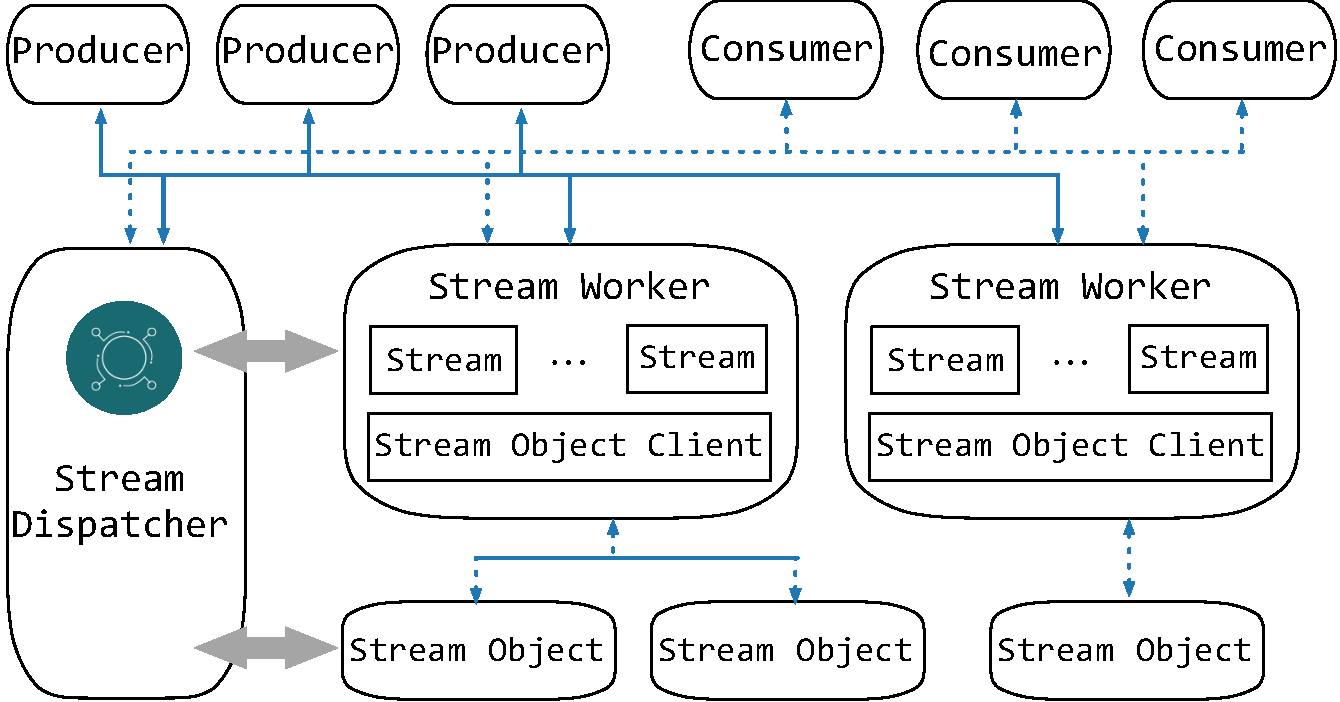
\includegraphics[scale=0.36]{figures/streamservice}
	\centering
	\vspace{-1em}
	\caption{Write Message to \sys.}
	\label{fig:service}
	\vspace{-1em}
\end{figure}

\noindent\underline{\textit{Producers and Consumers.}} Producers are responsible for publishing messages to topics, which are named resources for categorizing streaming messages. Consumers, located downstream, subscribe to these topics to receive and process the published messages. To ensure seamless integration with existing open-source message streaming services used by our customers in production environments, the producer and consumer message APIs are designed to be compatible with the open-source de facto standard. This maximizes connectivity with the ecosystem, allowing users to easily migrate their applications to \sys with minimum costs. Figure~\ref{fig:producer}  demonstrates the process of writing and reading messages using the producer and consumer APIs. In this example, a producer writes a new message ``Hello World'' as a key-value pair to a topic named ``\texttt{topic\_streamlake\_tes}''. The consumer then subscribes to this topic and processes published messages.

\begin{figure}[htbp]
	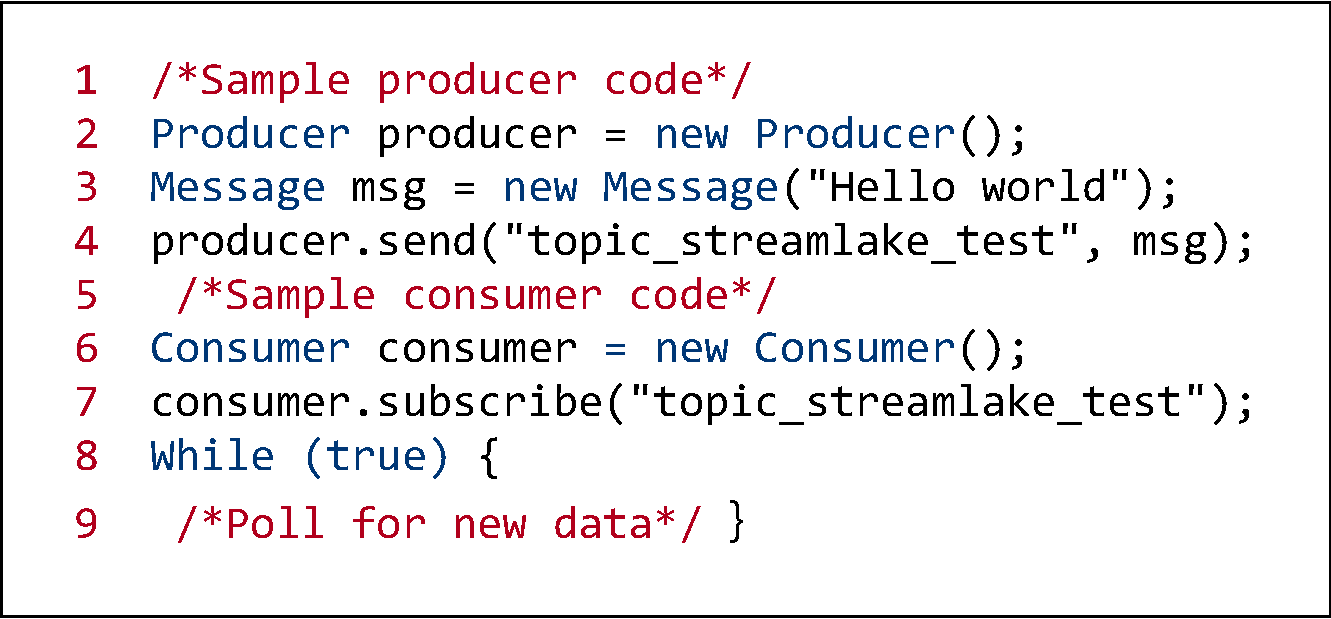
\includegraphics[scale=0.3]{figures/producer}
	\centering
	\vspace{-1em}
	\caption{Sample code of Producer and Consumer.}
	\label{fig:producer}
	\vspace{-1em}
\end{figure}

\noindent\underline{\textit{Stream workers}} work together with stream objects discussed in Section~\ref{subsec:streamobject} to tackle stream processing and message storage. The number of stream workers is determined by configurations and the physical resources allocated to the stream storage. Each stream worker is capable of handling multiple streams and a single stream object client. When a topic is created, streams are added to the stream workers in a round-robin manner to ensure even distribution and workload balancing across the cluster.

Each stream is mapped to a unique stream object in the storage layer, which is a  storage abstraction customized to  key-value message streaming. The stream object offers efficient interfaces and implementations for writing and reading streams from the storage pools. The persistence process is detailed in Figure~\ref{fig:write}.

The task of message delivery is carried out by stream object clients, which monitor the stream objects. These clients unwrap messages from clients, encapsulate them in the stream object data format, and redirect them to the corresponding stream objects via RDMA. To guarantee message delivery, the clients actively monitor the health of the stream objects to which they are connected and regularly exchange critical service data with the dispatcher service. This synchronization process includes reporting the health of the stream object connections and refreshing the stream objects connected to by the client.


\noindent\underline{\textit{Stream dispatcher.}} The stream dispatcher is responsible for managing the metadata and configurations of the messaging service, and directing external/internal requests to the appropriate resources for message  dispatch. The relationships among topics, streams, stream workers, and stream objects are stored as key-value pairs in a fault-tolerant key-value store within the stream dispatcher. When there is  a status change   (\eg a stream worker or topic is added or removed), the metadata  in the key-value store is updated immediately to refresh the topology tracking. This topology tracking aids the stream dispatcher in directing requests for message stream dispatch. When there is a producer or consumer connection request, the stream dispatcher will route the request to the appropriate stream worker based on the associated stream topic, establishing a direct message exchange channel between the producer, the stream worker, and the consumer.

\begin{figure}[htbp]
	\vspace{-1em}
	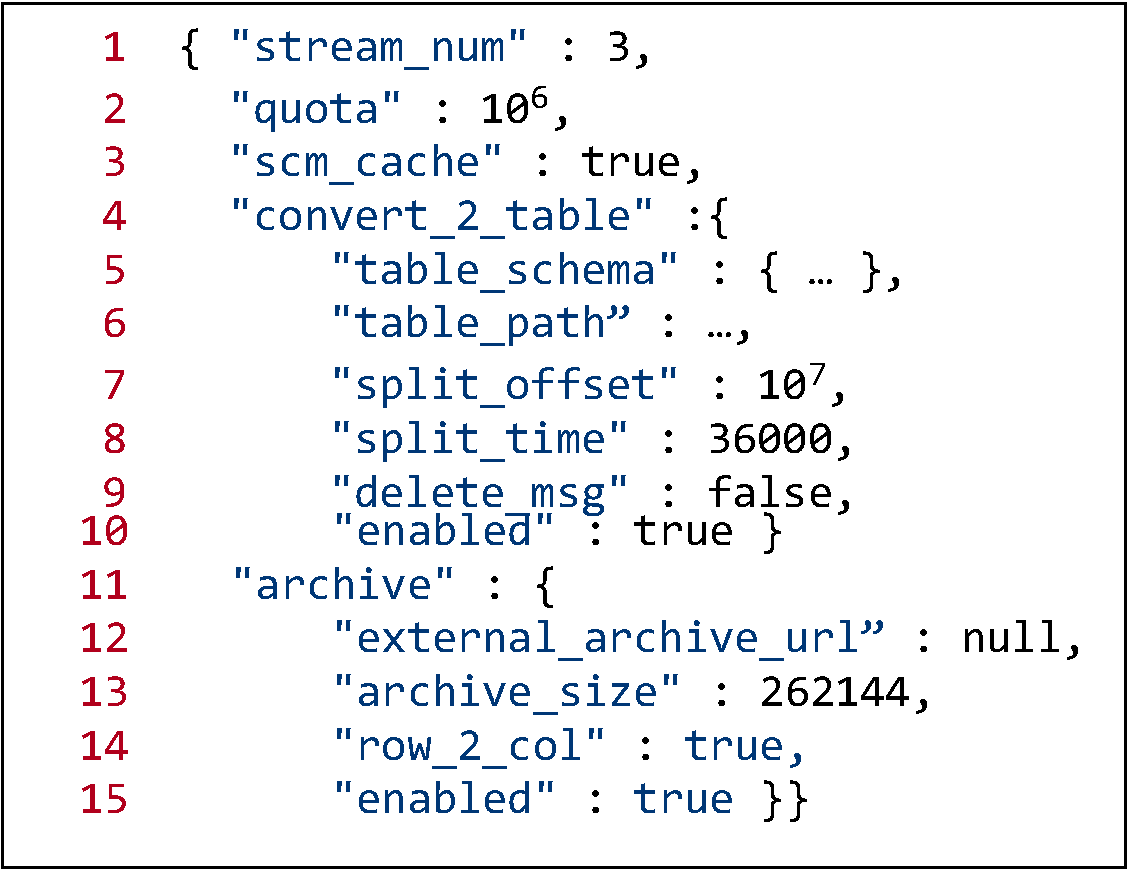
\includegraphics[scale=0.33]{figures/config}
	\centering
	\vspace{-1em}
	\caption{Stream Storage Configuration Example..}
	\label{fig:config}
	\vspace{-1.5em}
\end{figure}


The stream dispatcher also sets configurations for the messaging service in the unit of topic. An example of  configurations is shown in Figure~\ref{fig:config}.



$\bullet$~\textit{The \texttt{stream\_num} configuration} sets the parallelism of a topic, which should be provided during topic declaration. In the example, three streams are created for the topic and they are evenly distributed among stream workers to process messages in parallel.

$\bullet$~\textit{The \texttt{quota} configuration} sets the maximum processing rate for each stream. In the example, each stream can process up to $10^6$ messages per second.

$\bullet$~\textit{The \texttt{scm\_cache} configuration} enables the use of storage class memory (SCM) caches.

$\bullet$~\textit{The \texttt{convert\_2\_table} configuration} enables the automatic conversion of stream object messages to table object records, and it can also be converted back. When it is set, a background process will apply the \texttt{table\_schema} to convert messages to table object records periodically and save them in \texttt{table\_path}, \ie the table object directory. The conversion is triggered by either an accumulation of $10^7$ messages or the passing of 36000 seconds.  The advantage of this configuration will be illustrated in Section~\ref{subsec:lakehouse}.





$\bullet$~\textit{The \texttt{archive} configuration} automates the archiving of historical data to meet business and regulatory requirements. Data can be stored in the cost-effective \sys archive storage pool or automatically exported to an external storage system specified in the \textit{\texttt{external\_archive\_url} configuration}. The \textit{\texttt{archive\_size} configuration} denotes the data volume in MB that triggers archiving, and the \textit{\texttt{row\_2\_col} configuration} determines whether the data is archived in a columnar format. 

Overall, the \sys stream storage provides guaranteed delivery, efficient transfer, and high elasticity for enterprise use.

\noindent\textbf{Delivery Guarantee:} Our system ensures consistent message delivery through several measures. (1) Data within a stream object is strictly ordered, ensuring that messages are consumed in the order in which they are received. (2) Message writing is idempotent, which means that for network failure, duplicate messages sent by the producer  can be identified.
 (3) Strong data consistency is achieved by eliminating unreliable components like file systems and page caches, and storing data in  stream objects that can tolerant node, network, and disk failures. (4) The system provides exactly-once semantics through the use of a transaction manager and the two-phase commit protocol. This tracks participant actions and ensures that all results in a transaction are visible or invisible at the same time.
 
 %There are two typical scenarios. The first is that a producer writes a batch of messages to multiple streams. All messages are either successfully written or failed. The second scenario is that the application reads the message, processes the message, and writes the message to a new stream and the whole process are either successful or failed.

\noindent\textbf{Efficient Transfer:} Our system implements several mechanisms to efficiently transfer data. First, Stream workers and stream objects are connected through a data bus with RDMA, which reduces the switch overhead in the TCP/IP protocol stack. Second, an I/O aggregation mechanism is used to aggregate small I/O requests and increase throughput. This function can be disabled for latency-sensitive scenarios. Finally, a local cache is implemented at the stream object client to speed up message consumption.

\noindent\textbf{High Scalability:} Our system provides high elasticity by decoupling data storage and data serving to achieve high scalability. The number of stream workers can be adjusted without data migration, and the mapping between stream workers and stream objects can be updated to reflect the changes in a matter of seconds. This allows the message streaming service to easily scale up or down to accommodate changes in service demand.



\subsection{Lakehouse Read and Write}~\label{subsec:lakehouse}

 \sys also provides support for concurrent tabular data reads and writes, similar to  the architecture of lakehouse~\cite{}.
 Besides directly inserting tabular data, we can also get it from the conversion from streaming data.
  In this section, we first  describe the storage conversion from stream messages to tabular records, and then the implementation of key lakehouse operations.
 
 %insert table

\noindent \textbf{Stream-to-table conversion.} This process is performed by a background service and results in the conversion of records in stream objects to table objects, allowing for efficient downstream processing, which is triggered by the \texttt{convert\_2\_table} configuration in Figure~\ref{fig:config}, which include the table schema and time for data freshness in the downstream processing.  The table schema must be specified at the topic declaration, as it determines the expectations for field types and values across all messages. 
 To effectively leverage the storage, users  can choose to just retain messages in crucial topics as stream objects  to support real time applications while converting most stream data to table objects.  The reverse conversion, from table records to stream messages, is also supported for data playback. 
 %As shown in Figure~\ref{exp:fig:case} and Table~\ref{tab:case}, this design provides a good trade-off  between the system cost and latency, which also  helps to decouple the data processing from the business logics.
 This conversion helps to reduce the storage cost because we can just store one copy to achieve both stream and batch processing. Also, this design can reduce unnecessary data movement between the storage and compute clusters for data conversion.




For tabular data processing, our \sys services implement lakehouse read/write operations using a table object and high-performance caches to accelerate concurrent data reads and writes. In the rest of this subsection, we will introduce the implementation of key read/write operations in details.

\noindent \textbf{\texttt{CREATE TABLE:}} This operation begins by registering the table information, such as the schema, path, database, and table name, in the catalog. The \texttt{/data} and \texttt{/metadata} directories are then created under the table path. Then table configurations (schema, partition specification, target file size, etc.) are written to the metadata directory for persistence.



\noindent \textbf{\texttt{INSERT:}} This operation includes the persistence of data and metadata, as well as caching of metadata, which is introduced to combine small I/O accesses to the underlying storage pools.

\noindent \underline{\textit{(a) Data persistence:}} Records are written directly to the persistent layer as parquet files in the corresponding partition path under the table root directory.


%\cc{There seems should be an emphasize.}

\noindent \underline{\textit{(b) Metadata caching:}} Metadata updates are mostly small I/O operations. 
To avoid generating significant number of small files, we leverage a  write cache to aggregate the metadata updates, which is achieved through the following steps:
(b-1) Each added parquet file generates a commit record containing file-level metadata and descriptions. All new commit records are written to the write cache as key-value pairs when a commit is made.
(b-2) The latest snapshot will be read from the persistence layer to the cache and its commit data will be updated.
(b-3) The snapshot descriptions and version history in the catalog are also read from the persistence layer and  overwritten by adding the latest snapshot description. 

\noindent \underline{\textit{(c) Metadata persistence:}} Metadata in the  write cache is asynchronously flushed to the persistent storage pool when the buffer is full. A metadata management process (\texttt{MetaFresher}) transforms the commits and snapshots from key-value pairs to files and writes them to the \texttt{table/metadata} directory.

\begin{figure}[htbp]
	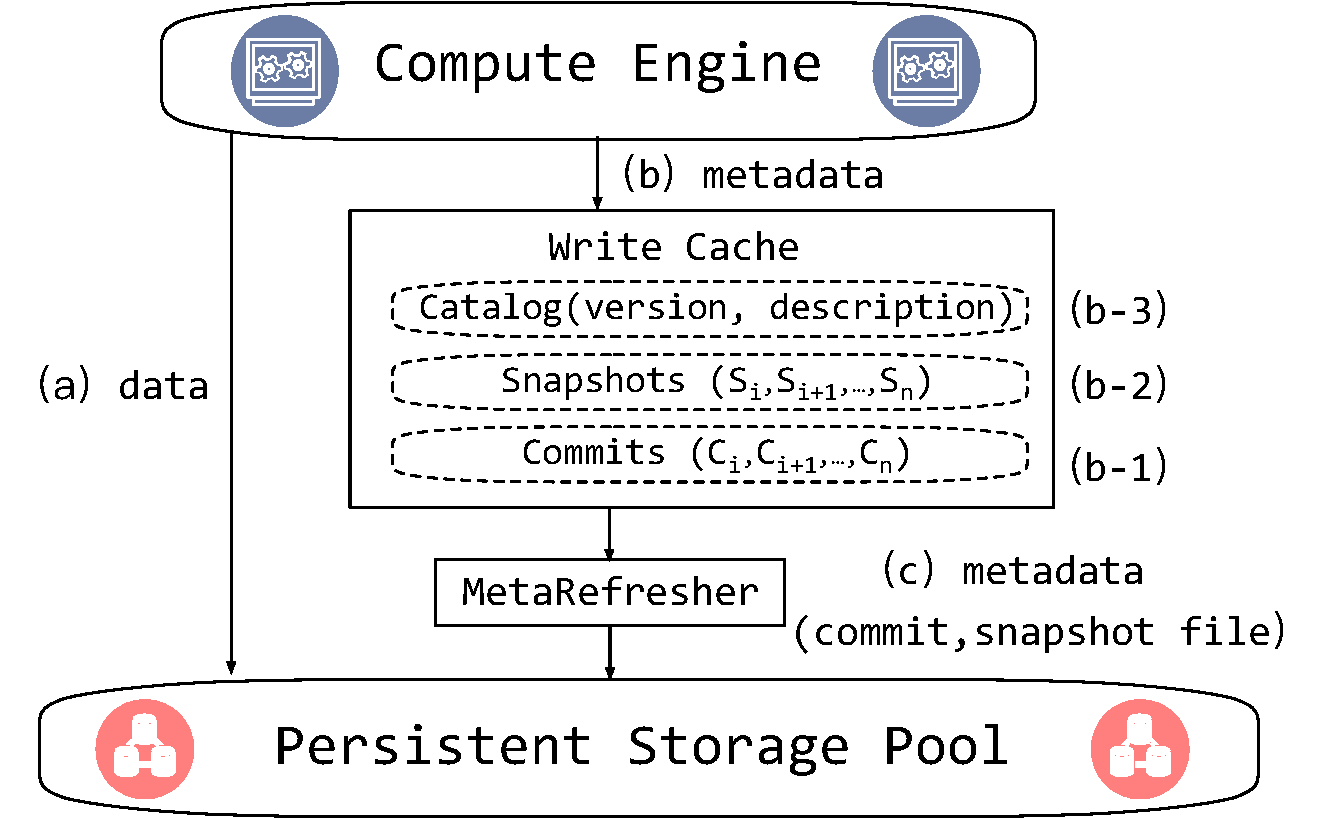
\includegraphics[scale=0.3]{figures/cache}
	\centering
	\vspace{-1em}
	\caption{Metadata Acceleration in Lakehouse Read/Write.}
	\label{fig:cache}
	\vspace{-1em}
\end{figure}


\noindent \textbf{\texttt{SELECT:}} The select operation first reads the catalog to retrieve the table profile for collecting the list of snapshot files needed for this query, such as the metadata version and snapshot descriptions. Then the corresponding snapshots and commit metadata are read from both the  cache and the persistent storage pool to generate the latest complete snapshots and commit metadata. When all the record file addresses are confirmed, data is read from the persistence pool by read tasks.

\noindent \textbf{\texttt{DELETE:}} The delete operation begins with a select operation to find files containing records that match the filtering conditions. There are two cases to consider:
If the filtering conditions match all data in several partitions, only the metadata will be updated, and a new commit version will be generated by eliminating the information of deleted partitions.
If the filtering conditions only match some files, these files will be read, and the data matching the filtering condition will be deleted. Computation pushdowns are applied to process file reads and writes to reduce data transmission to/from the compute engines.


\noindent \textbf{\texttt{UPDATE:}} Similar to the delete operation, update operation also uses a select statement to identify records that match the specified conditions. Optimizations, such as pushdowns, are applied to reduce data movements during the file read and write processes.

\noindent \textbf{\texttt{Drop Table:}} There are two types of drop table operations:
 (1) Drop table soft unregisters the table from the catalog but retains the table's metadata and data in the persistent layer for potential future restoration. To restore a soft-deleted table, a new table can be created and linked to the original table path, effectively registering the deleted table back to the catalog.
(2) Drop table hard  removes both the metadata (files under \texttt{/metadata}) and data (files under \texttt{/data}) of the table and clears the table from the catalog. Note that some of the metadata may have been written to the acceleration cache during the drop table hard operation and will be flushed to the persistent layer asynchronously in the background. The operation to delete the metadata will first clear it from the cache, and then delete it from the disk.

\subsection{Query Operator Computation Push Down}~\label{subsec:pushdown}




In this subsection, we introduce the computation pushdown (similar to S3 Select~\cite{s3}) to reduce the amount of data transfer between the  storage engine of \sys and the query engines.  Our pushdown method is built on top of an elastic, serverless engine in the data service layer. Here, we choose serverless computing as our execution model because it is lightweight  and flexible, which allows us to quickly start a large number of instances for computation tasks near the data sources, and free the resources as soon as the tasks are completed. The elasticity is important since CPU resources can be scarce during critical data management jobs.

The main components of the serverless function engine are shown in Figure~\ref{fig:serverless}, which include function dispatcher, worker instances, a worker manager, and a function repository. The function dispatcher schedules jobs and manages workflows, and worker instances execute the tasks. The worker manager oversees server resources and the life cycle of worker instances, and the function repository registers and stores function images. These modules work together to support elastic serverless computing.



\begin{figure}[htbp]
	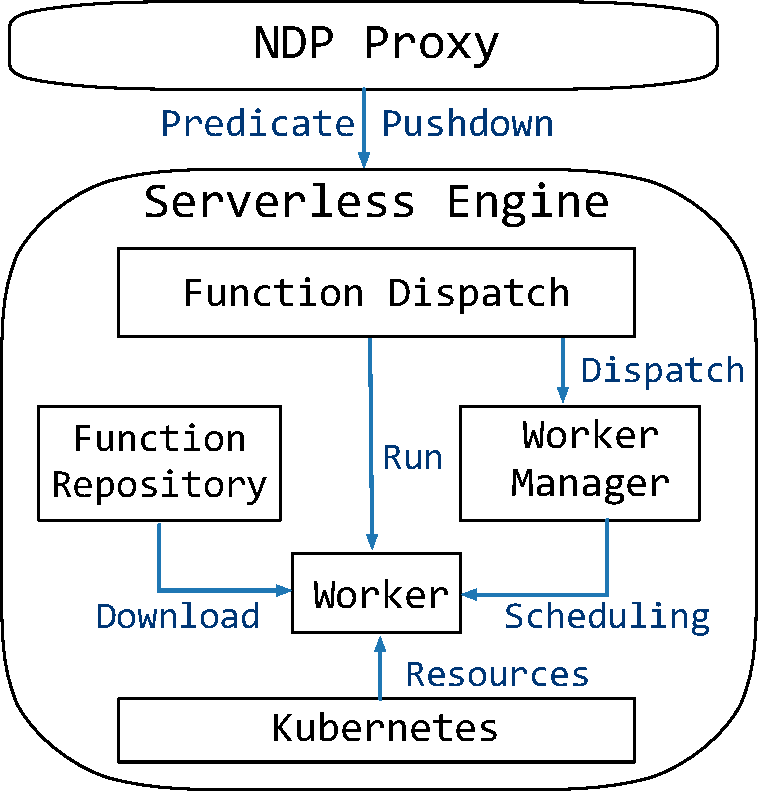
\includegraphics[scale=0.35]{figures/serverless}
	\centering
	\vspace{-1em}
	\caption{Serverless Function Engine.}
	\label{fig:serverless}
	\vspace{-1em}
\end{figure}

To be specific, when a job request is received, the function dispatcher obtains the data location from the storage devices and selects the appropriate storage nodes based on data distribution and available resources. The worker manager is then requested to deploy worker instances to the selected node. The worker instances download the necessary functions from the repository and execute the jobs using data from the storage infrastructure. Upon completion, a callback message is sent to the caller to notify them of the results. To ensure service quality, elastic scaling policies are used to dynamically adjust the number of nodes based on workload. 
For example, a \cc{load-balanced method} is used to balance scheduling among instances.


To achieve maximum pushdown benefits, three categories of query operators are supported, 

\begin{itemize}

\item \texttt{Projection Pushdown:}  Only selected columns will be returned.

\item \texttt{Filter Pushdown:} Only rows satisfying the filtering conditions will be returned.

\item \texttt{Aggregate  Pushdown:} The results of aggregate functions such as \texttt{Count}, \texttt{MAX} and \texttt{AVG} will be returned.

\end{itemize}

These operators are selected because the size of their output could be significantly smaller than the input, and thereby a large optimization opportunity can be achieved.
These query operators are implemented as separate functions, which are registered and executed in the serverless engine service. The implementation allows for sharing and reuse of the same query operator function by different query engines, as long as its image is registered in the serverless engine.


 %Finally, we build and open sourced plugins [14, 28] for popular big data engines such as Hive, Spark, and Presto [13, 32] to invoke query operator  pushdown. Users can easily install these plugins and speed up critical query processing

To facilitate the pushdown of query operators from the compute layer to the storage cluster in \sys, we have introduced the near data processing (NDP) Proxy and compute engine plugins for popular big data engines such as Hive, Spark, and Presto~\cite{hive, spark,presto} to invoke query operator  pushdown. 
 During query planning, the optimizer of  query  identifies operators that can be pushed down and sends the information to the NDP Proxy.  Then the NDP Proxy inserts these requests into a queue for traffic control and then sends them to the serverless engine for execution as shown in Figure~\ref{fig:serverless}.
As soon as the query results are ready, the NDP Proxy transfers them back to the compute engine using the high-speed data exchange bus of \sys, so as to ensure efficient data transfer.
Overall,  this process leverages the flexibility and elasticity of serverless computing, which allows for efficient use and release of server resources as required, resulting in better overall performance and resource utilization. 
%In addition, inspired by  methods proposed by~\cite{xiangyou, napa}, query operator pushdown can be used together with materialized views as cache to further optimize query performance.  This feature is on the roadmap to add to  \sys. 





%xiangyao yu



















